\state{Landau theory of phase transitions}{
	A ferroelectric crystal is one that supports a macroscopic polarization $P$, which usually arises because the underlying crystal structure does not have inversion symmetry.  However, as temperature or pressure is changed, the crystal may recover the inversion symmetry.  This can be modeled by Landau's theory of second order phase transitions, where we postulate a form for the free energy density (per unit volume)
	\eqn{given2}{
		\cF = \frac{a}{2} P^2 + \frac{b}{4} P^4 + \frac{c}{6} P^6 + \cdots,
	}
	where the coefficient $a = \ao (T - \Tc)$ is temperature dependent and all the other coefficients are constant.  Although the polarization $P$ is of course a vector, we assume that it can point only in a symmetry direction of the crystal, and so it is replaced by a scalar.
}

\prob{
	Assume that $b > 0$ and $c = 0$.  Use Eq.~\refeq{given2} to determine the form for the equilibrium $\PT$.
}

\sol{
	When $b > 0$ and $c = 0$, Eq.~\refeq{given2} becomes
	\eq{
		\cF = \frac{a}{2} P^2 + \frac{b}{4} P^4.
	}
	The equilibrium $\PT$ occurs at the minima of $\cF$, where $\dv*{\cF}{P} = 0$~\cite{Ferroelectricity}:
	\eq{
		\dv{\cF}{P} = a P + b P^3 = 0.
	}
	This implies
	\al{
		P &= 0, &
		P &= \pm \sqrt{-\frac{a}{b}}.
	}
	Note, however, that $P = 0$ is a local maximum of $\cF$ if $T < \Tc$:
	\eq{
		\left. \dv[2]{\cF}{P} \right|_{P = 0} = \brac{ a + 2 b P^2 }_{P = 0}
		= \ao (T - \Tc)
		< 0 \quad \text{when } T < \Tc.
	}
	However, the nonzero solution is imaginary for $T > \Tc$.  Thus the equilibrium $\PT$ is given by
	\eqn{PT}{
		\ans{ \PT = \begin{cases}
			\pm \sqrt{\dfrac{\ao}{b} (\Tc - T)} & T < \Tc, \\[2.5ex]
			0, \pm \sqrt{\dfrac{\ao}{b} (\Tc - T)} & T > \Tc.
		\end{cases} }
	}
	\vfix
}



\prob{
	Including in $\cF$ the energy of the polarization coupled to an external electric field $E$, determine the dielectric susceptibility $\chi = \dv*{P}{E}$ both above and below the critical temperature.
}


\sol{
	With the addition of the coupling term~\cite{Ferroelectricity}:
	\eq{
		\cF = \frac{a}{2} P^2 + \frac{b}{4} P^4 - E P.
	}
	Then
	\eqn{Fb}{
		\dv{\cF}{P} = a P + b P^3 - E
		= 0.
	}
	Differentiating both sides by E, we find
	\eq{
		0 = a \dv{P}{E} + b \dv{P^3}{E} - 1
		= a \dv{P}{E} + b \dv{P^3}{P} \dv{P}{E} - 1
		= a \chi + 3 b P^2 \chi - 1,
	}
	which implies
	\eqn{chiT}{
		\chiT = \begin{cases}
			\dfrac{1}{a + 3 b P^2}
			= \dfrac{1}{\ao (T - \Tc) + 3 \ao (\Tc - T)}
			= \ans{ \dfrac{1}{2 \ao (\Tc - T)}, } & \ans{ T < \Tc, } \\[2.5ex]
			\dfrac{1}{a}
			= \ans{ \dfrac{1}{\ao (T - \Tc)}, } & \ans{ T > \Tc, }
		\end{cases}
	}
	where we have used $\PT$ as defined in Eq.~\refeq{PT} and ignored the imaginary $\PT$.  Although this $\PT$ is evaluated at $E = 0$, we assume the difference is negligible from $\PT$ evaluated at small $E$, as mentioned on p.~79 of the lecture notes.
}



\prob{	\label{2c}
	Sketch curves for $\PT$, $\chiinvT$, and $\chiT$.
}

\sol{
	Figure~\ref{f2c} shows the curves of $\PT$~(top), $\chiinvT$~(bottom left), and $\chiT$~(bottom right).

	\begin{figure}[t] \centering
		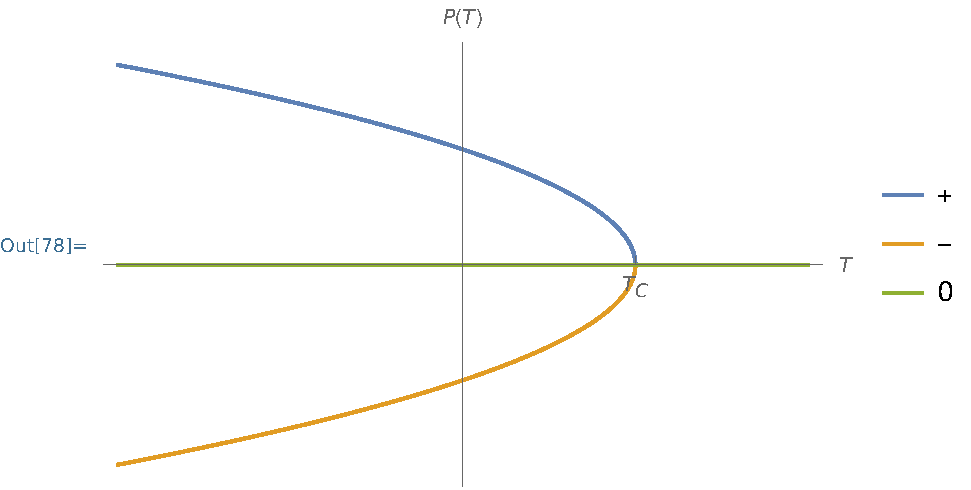
\includegraphics[width=0.49\textwidth,trim=1.5cm 0 0 0,clip]{2ci} \\[0.5cm]
		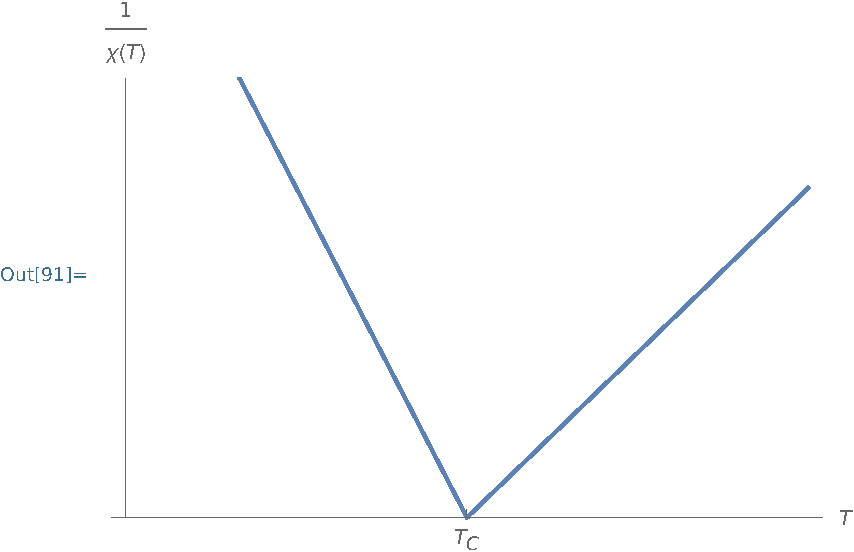
\includegraphics[width=0.43\textwidth,trim=1.5cm 0 0 0,clip]{2cii} \hspace{1cm}
		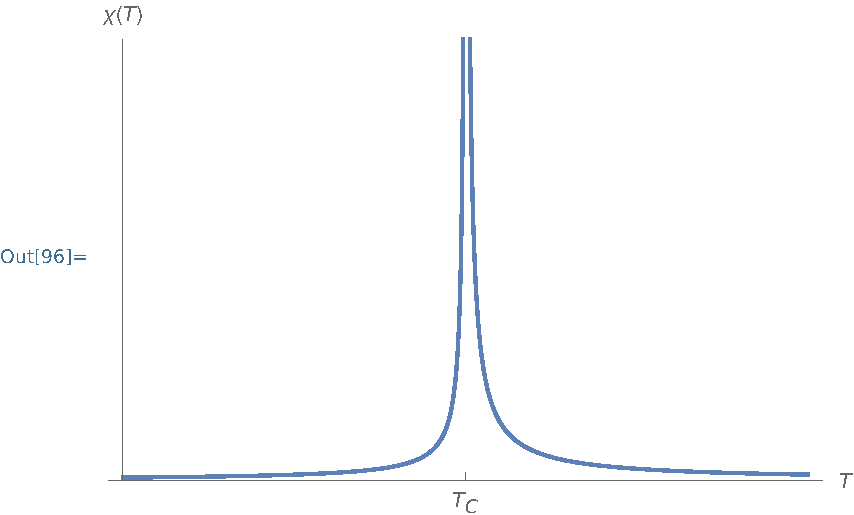
\includegraphics[width=0.43\textwidth,trim=1.5cm 0 0 0,clip]{2ciii}
		\caption{Plots of $\PT$~(top), $\chiinvT$~(bottom left), and $\chiT$~(bottom right), where $\PT$ is given by Eq.~\refeq{PT} and $\chiT$ is given by Eq.~\refeq{chiT}.  In the top figure, the blue~(gold) line corresponds to the upper~(lower) sign, and the green line to 0.}
		\label{f2c}
	\end{figure}
}



\prob{	\label{2d}
	In a different material, the free energy is described by a similar form to Eq.~\refeq{given2}, but with $b < 0$ and $c > 0$.  By sketching $\cF$ at different temperatures, discuss the behavior of the equilibrium polarization and the linear susceptibility, contrasting the results with those found in \ref{2c}.
}

\sol{
	$\cF$ is shown for at temperatures above, equal to, and below the critical temperature for the current case in Fig.~\ref{f2d}~(left) and for the case of \ref{2c} in Fig.~\ref{f2d}~(right).
	
	Equilibrium polarizations occur at the local minima of $\cF(P)$.  In the $b < 0$, $c > 0$ case, there are three equilibrium polarizations when $T > \Tc$ and two when $T \leq \Tc$.  In the $b > 0$, $c = 0$ case, there is one equilibrium polarization at $P = 0$ when $T \geq \Tc$ and two when $T < \Tc$.  The behavior in the former case is signifies a first-order phase transition, since $P$ acquires a nonzero value immediately below the critical temperature~\cite[p.~556]{Ashcroft}.
	
	In the $b > 0$, $c = 0$ case, the susceptibility diverges at the critical temperature as seen in Fig.~\ref{f2c}~(bottom right).  This is characteristic of a second-order phase transition as stated on p.~79 of the lecture notes.  In the $b < 0$, $c > 0$ case, the susceptibility is discontinuous but does not diverge.
	
	\begin{figure}[t] \centering
		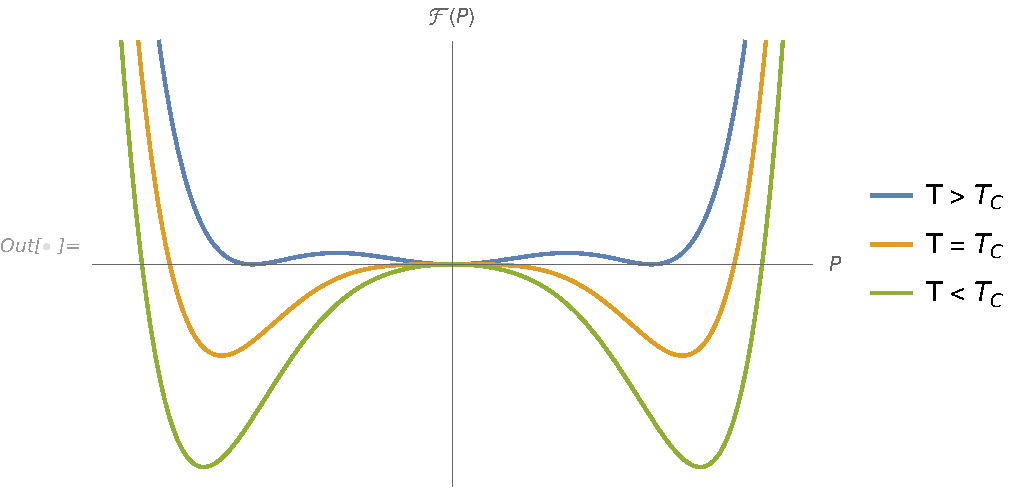
\includegraphics[width=0.49\textwidth,trim=1.5cm 0 0 0,clip]{2d} \hfill
		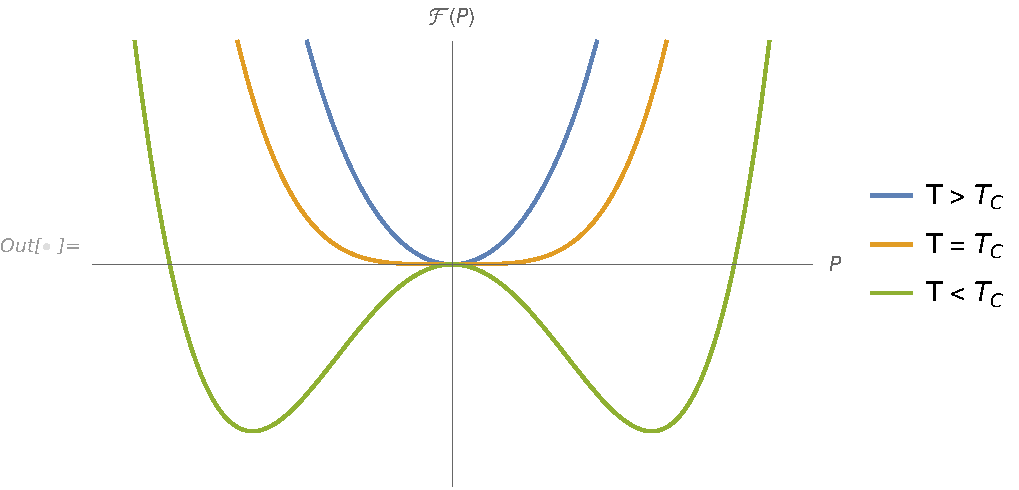
\includegraphics[width=0.49\textwidth,trim=1.5cm 0 0 0,clip]{2d2}
		\caption{Plots of $\cF(P)$ for the material of \ref{2d} with $b < 0$ and $c > 0$~(left) and for the material of \ref{2c} $b > 0$ and $c = 0$~(right).  Curves are shown for $T > \Tc$~(blue), $T = \Tc$~(gold), and $T < \Tc$~(green).}
		\label{f2d}
	\end{figure}
}